\chapter{Method}%
\label{ch:method}

In this chapter we introduce the theoretical idea of our Bayesian modeling of source separation. First we explicitly state our chosen model of the problem, next derive a suitable optimization objective from it and then explain how we can optimize towards that.

We propose the graphical model as shown in \cref{fig:graphical_model} as the generative story of music tracks being generated from separate source tracks. For each source a sample is taken from the latent source distribution. The observed mix is generated deterministically from the full set of sources. Without loss of generality we fix this function to be the mean.

\begin{marginfigure}[-15em]
    \begin{tikzpicture}
    \node[obs]                (x) {\(\x\)};
    \node[latent, left=of x]  (z) {\(\z\)};

    \edge {z} {x} ; %

    \plate {xz} {(x)(z)} {\(N\)} ;
\end{tikzpicture}
%
    \caption{The used graphical model for the source separation task. We have the latent source channel variables \(\s_k\). Exemplary here, as in our data, we have four sources. The mix \(\m\) is observed.}%
    \label{fig:graphical_model}
\end{marginfigure}

Our stated task in \sref{ch:question} is to retreive the sources \(\{\s_1,\…,\s_N\}\) from a given mix \(\m\). Our model is trained without using sample tuples \[(\m, \{\s_1,\…,\s_N\}): f(\{\s_1,\…,\s_N\}) = \m\] which would show the relation between separate sources and mixes. The general idea is visualized in \cref{fig:method}.

\begin{figure}[t]
    \begin{tikzpicture}
    % Second column, prior dstirbutions
    \node (d0) {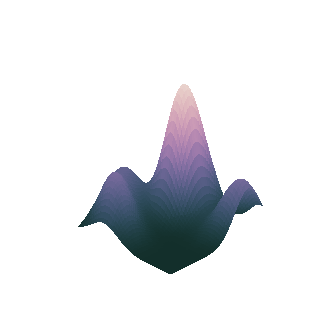
\includegraphics[width=40pt]{dist_0}};
    \node[below=-10pt of d0] (d1) {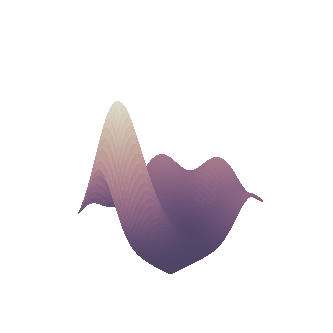
\includegraphics[width=40pt]{dist_1}};
    \node[below=-10pt of d1] (d2) {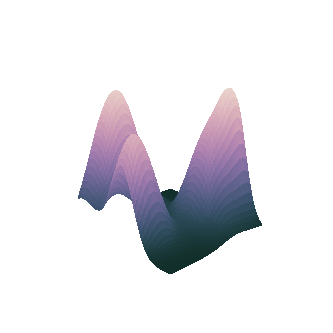
\includegraphics[width=40pt]{dist_2}};
    \node[below=-10pt of d2] (d3) {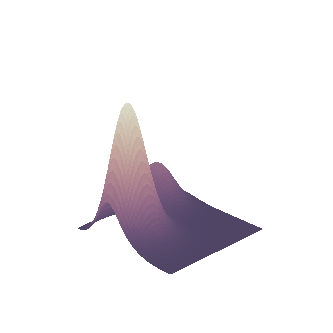
\includegraphics[width=40pt]{dist_3}};
    \node[above=-9pt of d0] (td) {\(p(\s_i)\)};

    % First columns, data
    \node[left=30pt of d0] (s0) {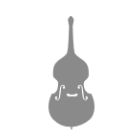
\includegraphics[width=25pt]{mixing/bass.png}};
    \node[left=30pt of d1] (s1) {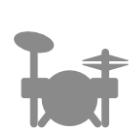
\includegraphics[width=25pt]{mixing/drums.png}};
    \node[left=30pt of d2] (s2) {
\includegraphics[width=25pt]{mixing/voice.png}};
    \node[left=30pt of d3] (s3) {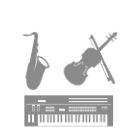
\includegraphics[width=25pt]{mixing/other.png}};
    \node[above=0pt of s0] (ts) {data};

    % Arrows frist to second
    \draw [->] (s0) to (d0);
    \draw [->] (s1) to (d1);
    \draw [->] (s2) to (d2);
    \draw [->] (s3) to (d3);
    \draw (ts) -- (td) node [above, midway,align=center] {estimate};

    % Column posterior
    \node[right=30pt of d0] (dp0) {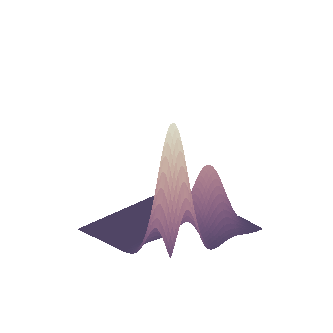
\includegraphics[width=40pt]{dist_0_post}};
    \node[right=30pt of d1] (dp1) {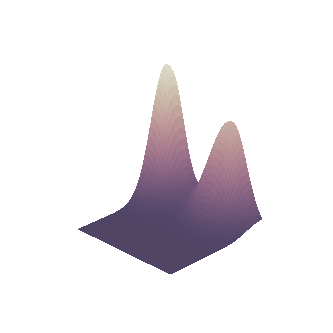
\includegraphics[width=40pt]{dist_1_post}};
    \node[right=30pt of d2] (dp2) {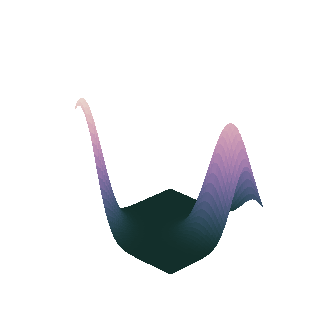
\includegraphics[width=40pt]{dist_2_post}};
    \node[right=30pt of d3] (dp3) {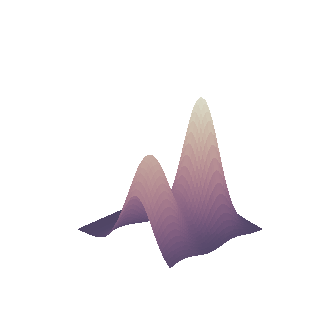
\includegraphics[width=40pt]{dist_3_post}};
    \node[above=0pt of dp0] (tp) {posterior};

    % Mix wave
    \node[above right=10pt of td] (wav) {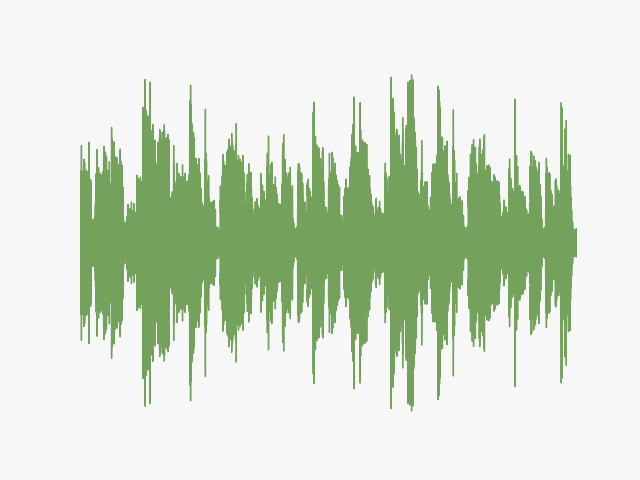
\includegraphics[width=40pt]{mixing/mix_wav.png}};
\end{tikzpicture}

    \caption{The method visualized}
    \label{fig:method}
\end{figure}

Looking back at the graphical model in \cref{fig:graphical_model}, it implies the following factorization:

\begin{align}
    p(\m)
    &= \∫^N p(\s_1,\…,\s_N,\m) \,d^N \s\\
    &= \∫^N p(\m | \s_1,\…,\s_N) \· p(\s_1,\…,\s_N) \,d^N \s\\
    &= \∫^N p(\m | \s_1,\…,\s_N) \· p(\s_1) \cdots p(\s_N) \,d^N \s
\end{align}

While the conditional \(p(\m | \s_1,\…,\s_N)\) is not even probabilistic, as the mix is generated deterministically as the mean of the sources, the model posterior \(p(\s_1,\…,\s_N | \m)\) is intractable and precisely what we are interested in. Again we want to make it clear that this setup changes the typically optimization target, as seen in other source separation approaches. We factorize the distribution \(p(\m)\) of mixed songs, with the intention of then extracting the most likely \I{latent} components that generate this mix, the sources.

Already with the graphical model we introduce a fairly big assumption, namely that we can model the source distributions independently from each other when modeling the joint:

\begin{align}
    p(\m,\s_1,\…,\s_N) &\equiv p(\m|\s_1,\…,\s_N) \· \Π_k^N p(\s_k)
\end{align}

It is intuitive that this assumption does not, in general, hold for the musical domain. We can expect a different behaviour for a \I{guitar} in a song involving a second source like a \I{percussion set}. The joint of those two models is different than their independent densities~\footnote{A practical counter-example: If learning the behaviour of drums, only from solo drum recordings, one will encounter complex rhytms and sounds. In many rock genres drums often exhibit simpler sounds, providing beat and tempo. These two distributions are not the same.}. Nevertheless this assumption is crucial to be able to model the prior instrumental models without needing the tuples \((\s_1,\…,\s_N)\) of co-occurring stems.

The general process is as follows:

First, because we assumed in our graphical model the latent sources to be independent, there exists a probability distribution \(p(\s_k)\) for each source \(k\). Thereout we need to choose a model which gives the parametrized approximated prior \(p_{\B{\θ}}(\s_k)\) with the parameters \(\B{\θ}\) which we optimize with the samples from \(\mathcal{D}_k\).

Second, for each source there exists a posterior given a mix \(p(\s_k | \m)\) from which we want to draw samples. Here two approaches are possible. Either we can propose a approximate posterior \(\aprxpost\), which is trained to minimize the divergence from the previously trained and fixed corresponding prior (VAE setting). Or, we can sample directly from the posterior using Stochastic Gradient Langevin Dynamics (SGLD)~\cite{wellingBayesian2011} without explicitly approximating the posterior distribution (sampling setting). Both optimization, either training or sampling, happen under the mixing constraint:

\begin{align}
    \Σ_{k=1}^N \s_k = \m
\end{align}

When using the VAE setting we then can sample from each posterior to retreive a set of (approximately) correct source tracks. In the case of using Langevin dynamics the iterative sampling will directly give this set from the prior distributions.

Thinking in the common terms of the VAE we need to choose:

\begin{enumerate}
    \item a parametrization \(p_{\B{\θ}}(\s_k)\) of the \I{prior} distribution
    \item a parametrized approximate posterior distribution \(\aprxpost\) with parameters \(\B{\η}\)
    \item a parametrized \I{encoder} which gives the parameters for the posterior distribution \(\texttt{Encoder}_{\B{\φ}}(\m) = \B{\η}\)
    \item a \I{decoder} which returns the input \(\m\) from the latents \linebreak \({\texttt{Decoder}(\{\s_1,\…,\s_N\}) = \m}\)
\end{enumerate}

As stated before the decoder in our case is the mean function, thus not probabilistic and without parameters. It is certainly possible to parametrize the decoder with trainable parameters. This would imply though that the latent samples are not in the \I{direct form} of the source sounds but under a (unkown) transformation.

\section{Modeling the priors}
The first step in the training procedure is the training of the independent source priors \(p(\s_k)\). We have to choose a model for estimating the density that results in smooth, tight densities but also is capable enough to capture the complex data space of audio data. We choose to estimate the priors with flow models for which we gave an overview in \cref{sub:flows}. For different representation of the input different network architectures are mode suited. We experiment both with inputing directly the time-domain wave but also modeling on top of a spectral transformation of the time-domain data.

The two main variants of normalizing flows we build our priors from are the RealNVP and Glow. Their most important difference is the different formulation of the coupling layers. For the coupling layers we have to split the layer input into two equally sized subsets, one of whom will be transformed using an invertable transformation parametrized by the other. The RealNVP masks the data spatially or over the channels. When done spatially a checkerboard binary mask is used (same for all channels), for the channel variant the channels are assigned in a even-odd switching. Glow on the other hand learns a \(1\× 1\)-convolution which permutes the data channel-wise and than just splits the data along the channel dimension into two. For both RealNVP and Glow prior works exists adapting the architecture specifically to the time-series domain by integrating WaveNet modules, FloWaveNet~\cite{kimFloWaveNet2019a} and WaveGlow~\cite{prengerWaveGlow2018}, respectively. \itodo{wat about waveflow}

For the case of the time-domain representation, the data has only one channel (mono-audio). Therefore a Glow-like shuffleing of channels is not possible and we resort to using spatial masking for the coupling layers. A one-dimensional mask is used over the time dimension. In the case of using a spectral representation of the audio data, the input samples have a lower time resolution but instead the frequency distribution over a deeper channel dimension. Therefore we can also experiment with channel-shuffleing.

\section{Sampling from the posteriors}
After having estimated the \(N\) prior distributions the first possiblity for retreiving sample estimates \(\s_k\) is sampling from the posterior using Langevin dynamics~\cite{nealMCMC2012}. While it is a classical approach to stochastic modeling of a dynamical modelcular system, \textcite{wellingBayesian2011} has shown how to employ Langevin dynamics as an MCMC sampling process for sampling from the posterior in Bayesian modeling. With Stochastic Gradient Langevin Dynamics (SGLD) we can sample from \(\s_i \sim p(\· | \m)\) without computing, explicitly, the posterior \(p(\s_i | \m)\).

\itodo{explanation}

\begin{algorithm}
    \caption{Sampling from the posterior using SGLD}%
    \label{alg:vae}
    \begin{algorithmic}[1]
        \For{i=100}
        \EndFor%
    \end{algorithmic}
\end{algorithm}



The idea of using SGLD in combination with deep parametrized priors was, concurrently to this work, introduced in \textcite{jayaramSource2020}. The authors argue that direct optimization under the prior distribution is not successfull due to the severe peakedness of the priors. Thus, they argue, the stochasticity, added with the Gaussian noise in SGLD, is needed to not get stuck in local optimas under the manifold. We challenge that explanation as it is, blabla

{\color{red} I like the section so far, but I think you should emphasize more what are the challenges, e.g., for both the VAE approach and the Langevin dynamics we need a prior and a posterior. In addition, since we have a probabilistic approach we need to choose distributions for everything.}


\section{Modeling the posteriors}
We follow the same steps as previously shown for the latent variable models. First we introduce a approximate posterior \(\aprxpost\) for each source channel. Next we express the mix density as the expectation over those posteriors:

\begin{align}
    \log p(\m)
    &= \E_\aprxpost^N \left[ \log p(\m) \right]\label{eq:expectation_over_approx_post}
\end{align}

From here derive the ELBO in the same way as before, just now with \(N\) priors instead of one:

\begin{fullwidth}
    \newcommand{\post}{p(\s_1,\…,\s_N|\m)}
    \begin{align}
        \E_\aprxpost^N \left[ \log p(\m) \right]
        &= \E_\aprxpost^N \left[ \log \÷{p(\m,\s_1,\…,\s_N)}{\post} \right]\\
        &= \E_\aprxpost^N \left[ \log \÷{p(\m|\s_1,\…,\s_N) \· \Π_k^N p(\s_k)}{\Π_k^N \aprxpost} + \log \÷{\Π_k^N \aprxpost}{\post} \right]\\
        &\geq \Σ_k^N \E_\aprxpost \left[ \log \÷{p(\s_k)}{\aprxpost} \right]
             +\E_\aprxpost \left[ p(\m|\s_1,\…,\s_N) \right]\label{eq:final_elbo}\\
    \end{align}
\end{fullwidth}

Like in the VAE we now formulate the lower bound for approximting the graphical model with the approximate posterios \(\aprxpost\) which we will parametrize with deep neural networks. The source priors are estimated \I{a-priori} and  independtly and are also parametrized by neural networks.

Finally we note that this assumption is not being used for the independent approximate posteriors. While the true posterior certainly is the posterior of the joint source model, we choose our approximate posteriors to be independent. The expectation in \eqref{eq:expectation_over_approx_post} over those is still correct. The error arising from the independence assumption is captured in the thightness of the ELBO.

Assuming we have now a set of meaningful, discriminative priors \(p(\s_i)\) we need to combine the independent models to extract sources \(\{\s_i\}\) given a mix \(\m\). At the beginning of this section we already introduced the imagined generative model and derived the lower bound for the approximate posterior. Taking a step back again and looking at the posterior we have two general possibilities to retrieve samples from the posterior \(p(\s_i | \m)\).

\begin{align}
    p(\s_i|m)
    &= \÷{p(\m|\s_i)\· p(\s_i)}{p(\m)}
\end{align}

First we can model the approximate posterior \(\aprxpost\). By doing so we train a new subsequent function which directly retrieves the predicted sources given a mix. This method is, in principle, the same as we would see in a normal variational-autoencoder. Alternatively, finding the actual posterior to difficult to model, we can sample \(\s_i \sim p(\·|m)\) without computing the actual distribution.

\subsection{Variational-autoencoder}

\itodo{blabla}
